\chapter{Installation}
\label{sec:install}
% Old Ch. 1

\textit{Covered in \href{https://www.youtube.com/watch?v=oIsH0V3fRt8&list=PLjGmdnqrOKuYXiu7lgG5HW71jPEUd1XCm&index=2}{video 1 of the series}}
\vspace{6mm}

Probably the most complicated installation procedure you have ever seen, but I reassure you that it is worth the time. However, it is only a one-time process. Those are essential tools for you to code more advanced stuff using JavaScript. It is also a good practice in using the command line interface.

The hyperlinks to the resources needed are all clickable in this chapter.

\section*{For those of you not using Git}

You would still need to perform step \cref{sec:install1} if you are using a Windows machine.

You can download the code as a zip file \href{https://github.com/KidProf/static-web-sandbox}{by following this URL}.\footnote{Link: \url{https://github.com/KidProf/static-web-sandbox}} (see \cref{fig:githubzip}) You do not need a GitHub account to do so. 

After that, proceed with step \cref{sec:install5}, and unzip your code inside the folder, then proceed with steps \cref{sec:install7} and onwards.

\begin{figure}[h]
\centering
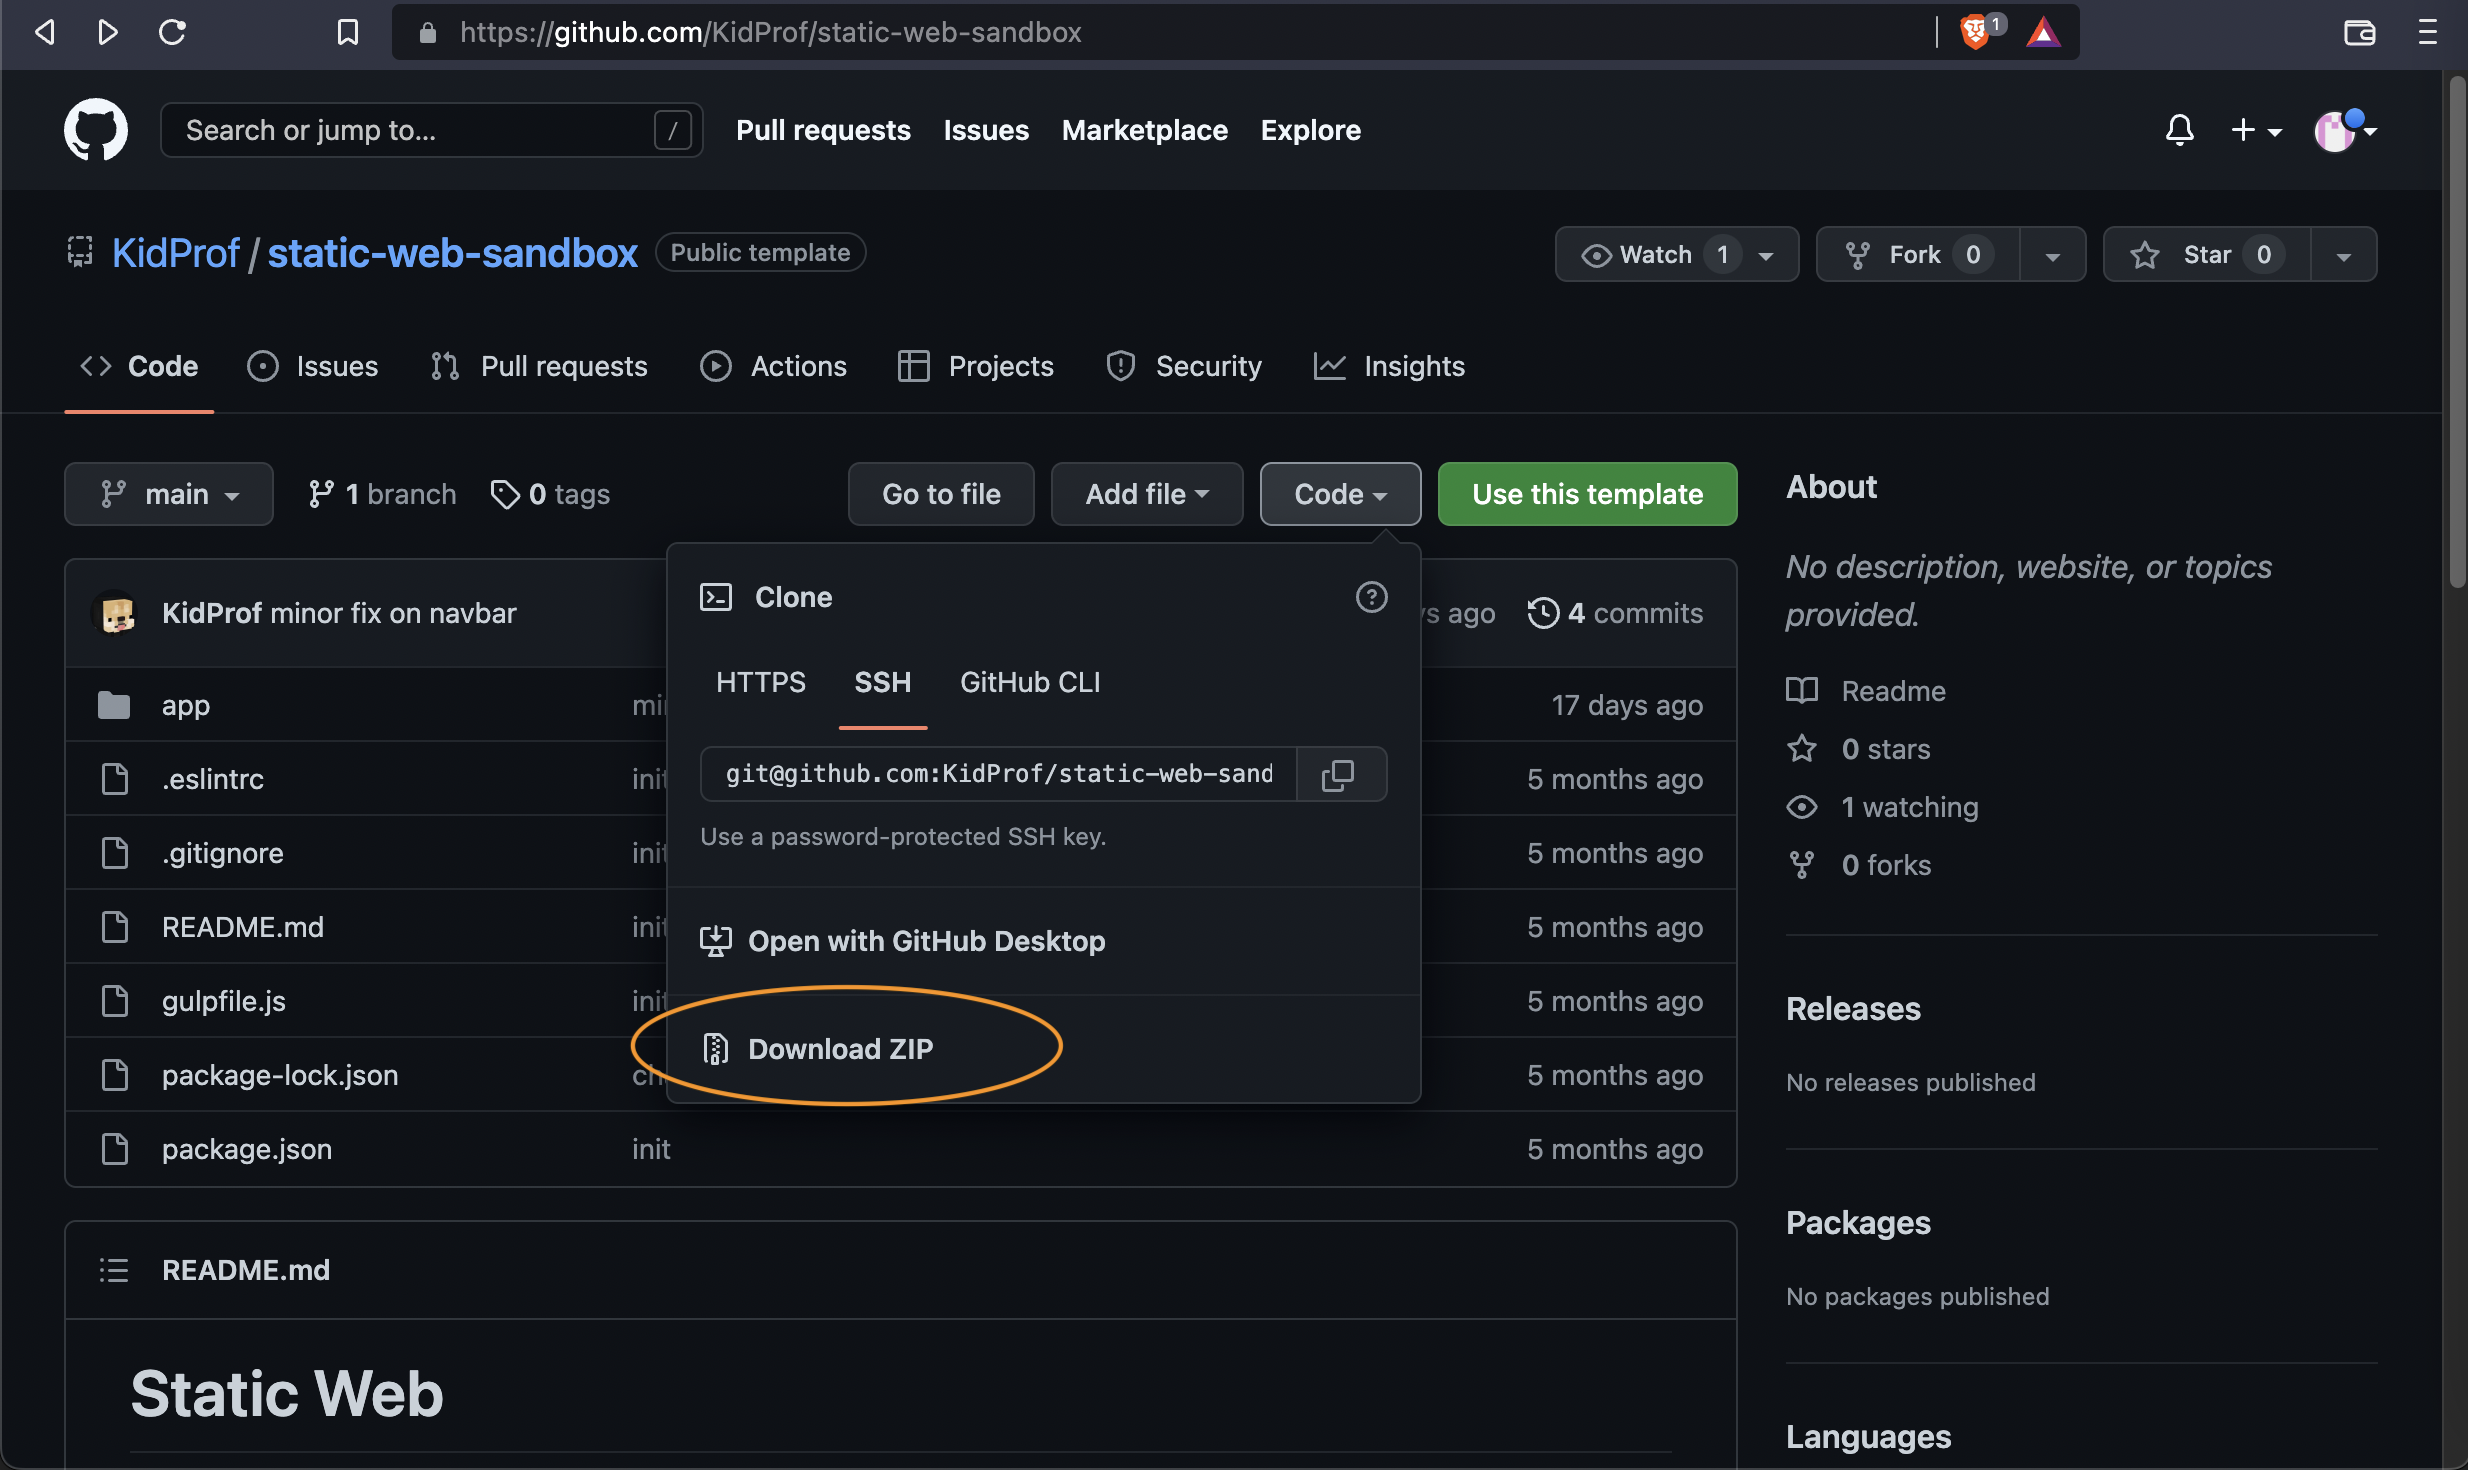
\includegraphics[width=15cm]{images/ch1-download-as-zip.png}
\caption{Screenshot from GitHub showing how to download the code by zip}
\label{fig:githubzip}
\end{figure}

\section{Git Bash (for Windows only)}
\label{sec:install1}

\textit{If you are using MacOS or Linux, skip to step \cref{sec:install2}}
\vspace{6mm}

For Windows users\footnote{This 'discrimination' is due to the fact that Windows CMD and PowerShell use slightly different command keywords compared to MacOS and Linux.}, you need to download Git Bash by following \href{https://git-scm.com/download/win}{this URL}.\footnote{Link: \url{https://git-scm.com/download/win}} 

\section{Creating a GitHub account}
\label{sec:install2}

\textit{If you have one then login to your account and proceed to step \cref{sec:install3}}
\vspace{6mm}

Create your own GitHub account \href{https://github.com/}{by following this URL}.\footnote{Link: \url{https://github.com/}} Remember the email you used for registration.

\section{Creating a new repository using the template}
\label{sec:install3}

Open my template by following \href{https://github.com/KidProf/static-web-sandbox}{this URL}.\footnote{Link: \url{https://github.com/KidProf/static-web-sandbox}} Then click the big green button \textit{Use this template} (you can also see it in \cref{fig:githubzip} (not the circled button but the big green one)). You will be prompted to create a new repository. \textbf{Repository} is a fancier word for project, sometimes abbreviated to \textbf{repo}. Provide a repository name (a.k.a. project name) of your choice, preferably something meaningful; and you can set it either to public or private based on your own preference. You can change these two settings in the future. Do not change up any other settings in this page. (see \cref{fig:createnewrepo})

\begin{figure}[h]
\centering
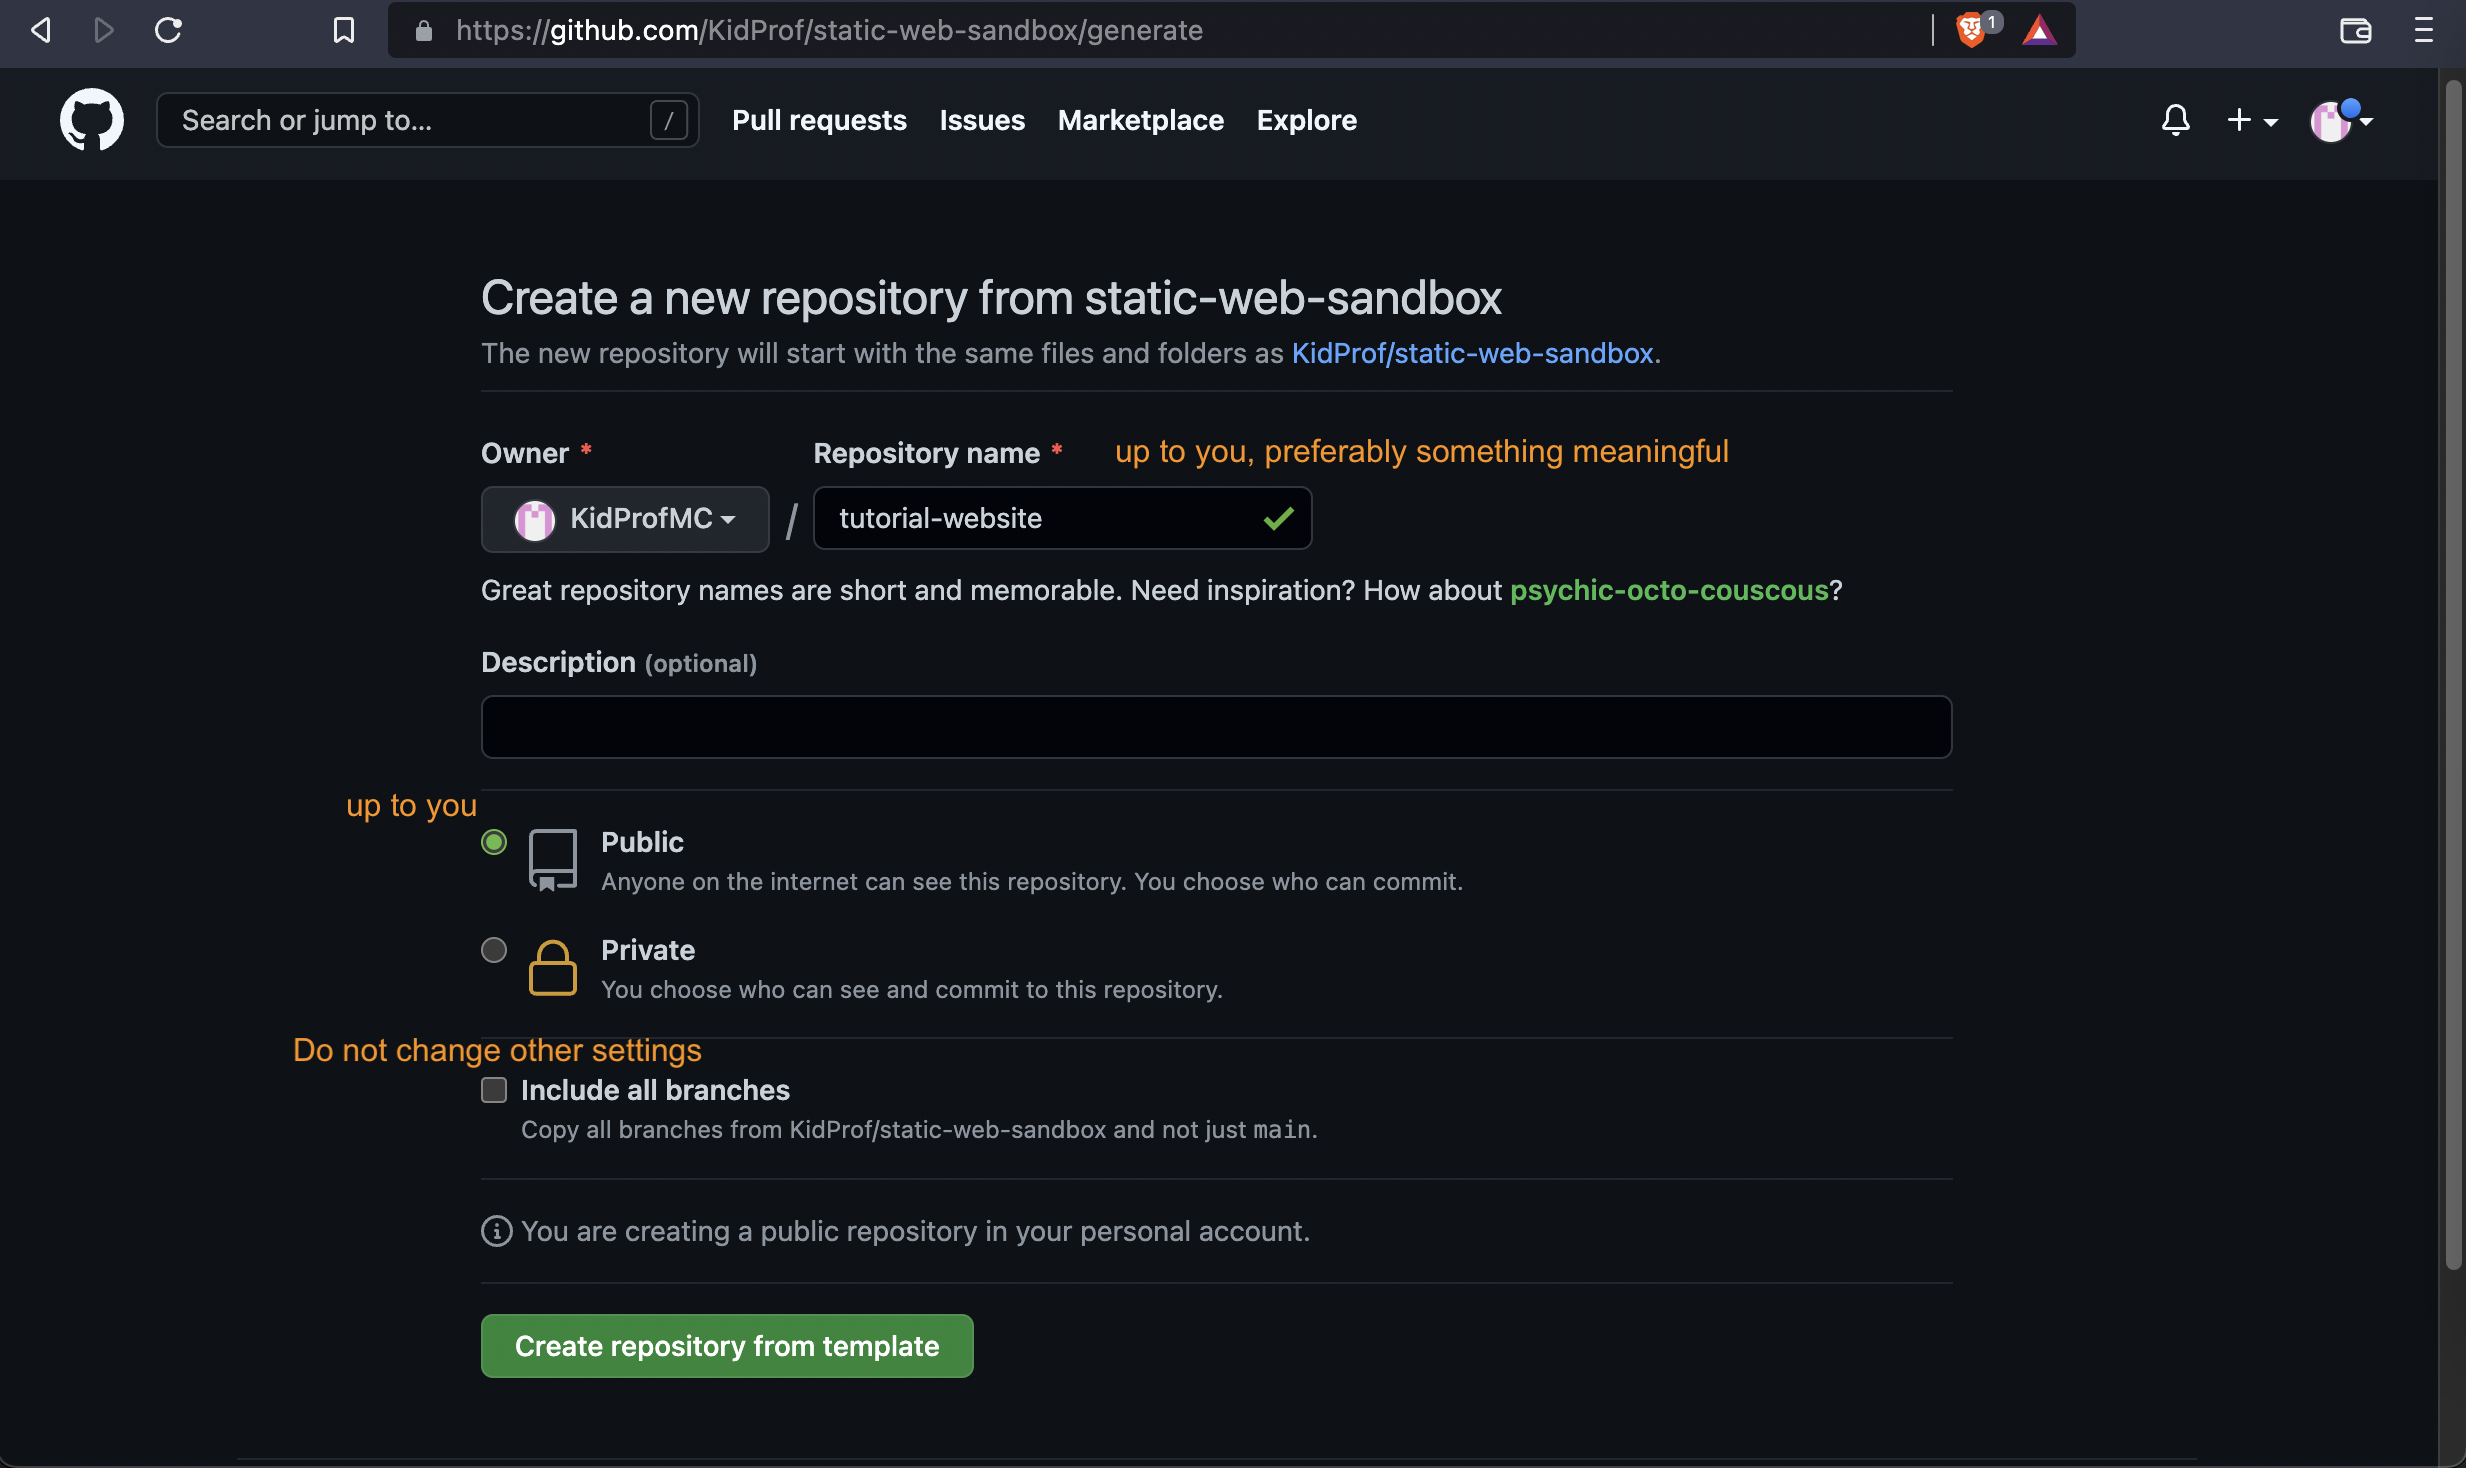
\includegraphics[width=15cm]{images/ch1-create-new-repo.png}
\caption{Creating a new repository}
\label{fig:createnewrepo}
\end{figure}

\section{Creating an SSH key}

An SSH key is to verify your identity on your local machine, so that you can access and manage your repositories on GitHub from your local machine.

Follow \href{https://docs.github.com/en/authentication/connecting-to-github-with-ssh/generating-a-new-ssh-key-and-adding-it-to-the-ssh-agent}{this tutorial}\footnote{Link: \url{https://docs.github.com/en/authentication/connecting-to-github-with-ssh/generating-a-new-ssh-key-and-adding-it-to-the-ssh-agent}}, then \href{https://docs.github.com/en/authentication/connecting-to-github-with-ssh/adding-a-new-ssh-key-to-your-github-account}{this tutorial}\footnote{Link: \url{https://docs.github.com/en/authentication/connecting-to-github-with-ssh/adding-a-new-ssh-key-to-your-github-account}}, and you are good to go. 
\vspace{6mm}

Use Git Bash if you are on a Windows machine, use the Terminal if you are on a MacOS machine, or use the Shell if you are on a Linux machine. There is no need to understand and remember the commands, copying and pasting is arguably one of the skills programmers need. \textbf{The \$ symbol indicates the start of a command, so you do not need to copy the \$ symbol.}
\vspace{6mm}

For example, if I am using a Windows machine, I would run the following set of commands in my Git Bash line by line. Remember to replace the email with your own email, the one you used to register for your GitHub account.

\begin{lstlisting}[language=bash]
$ ssh-keygen -t ed25519 -C "your_email@example.com"
$ eval "$(ssh-agent -s)"
$ ssh-add ~/.ssh/id_ed25519
$ clip < ~/.ssh/id_ed25519.pub
\end{lstlisting}

The \texttt{clip} command copies the things you need to your clipboard. You just need to paste it to the appropriate spot on the GitHub website according to the tutorials.

\section{Creating a folder using command line}
\label{sec:install5}

From now on, I would use the term \textbf{command line} to refer to Git Bash if you are on Windows, or the Terminal if you are on MacOS, or the Shell if you are on Linux. 

So now open the command line, use \texttt{mkdir} followed by a folder name to create a new folder to store your code. Then, use \texttt{cd} followed by the folder name to enter that folder.

\begin{lstlisting}[language=bash]
# KidProf in ~
$ mkdir code

# KidProf in ~
$ cd code

# KidProf in ~/code
$ 
\end{lstlisting}

\section{Downloading the code using SSH key}
\label{sec:install6}

Go back to your project on GitHub, click the big green button \textit{Code} (see \cref{fig:downloadbyssh}), then remember to select \textit{SSH}, then copy the URL given.

\begin{figure}[h]
\centering
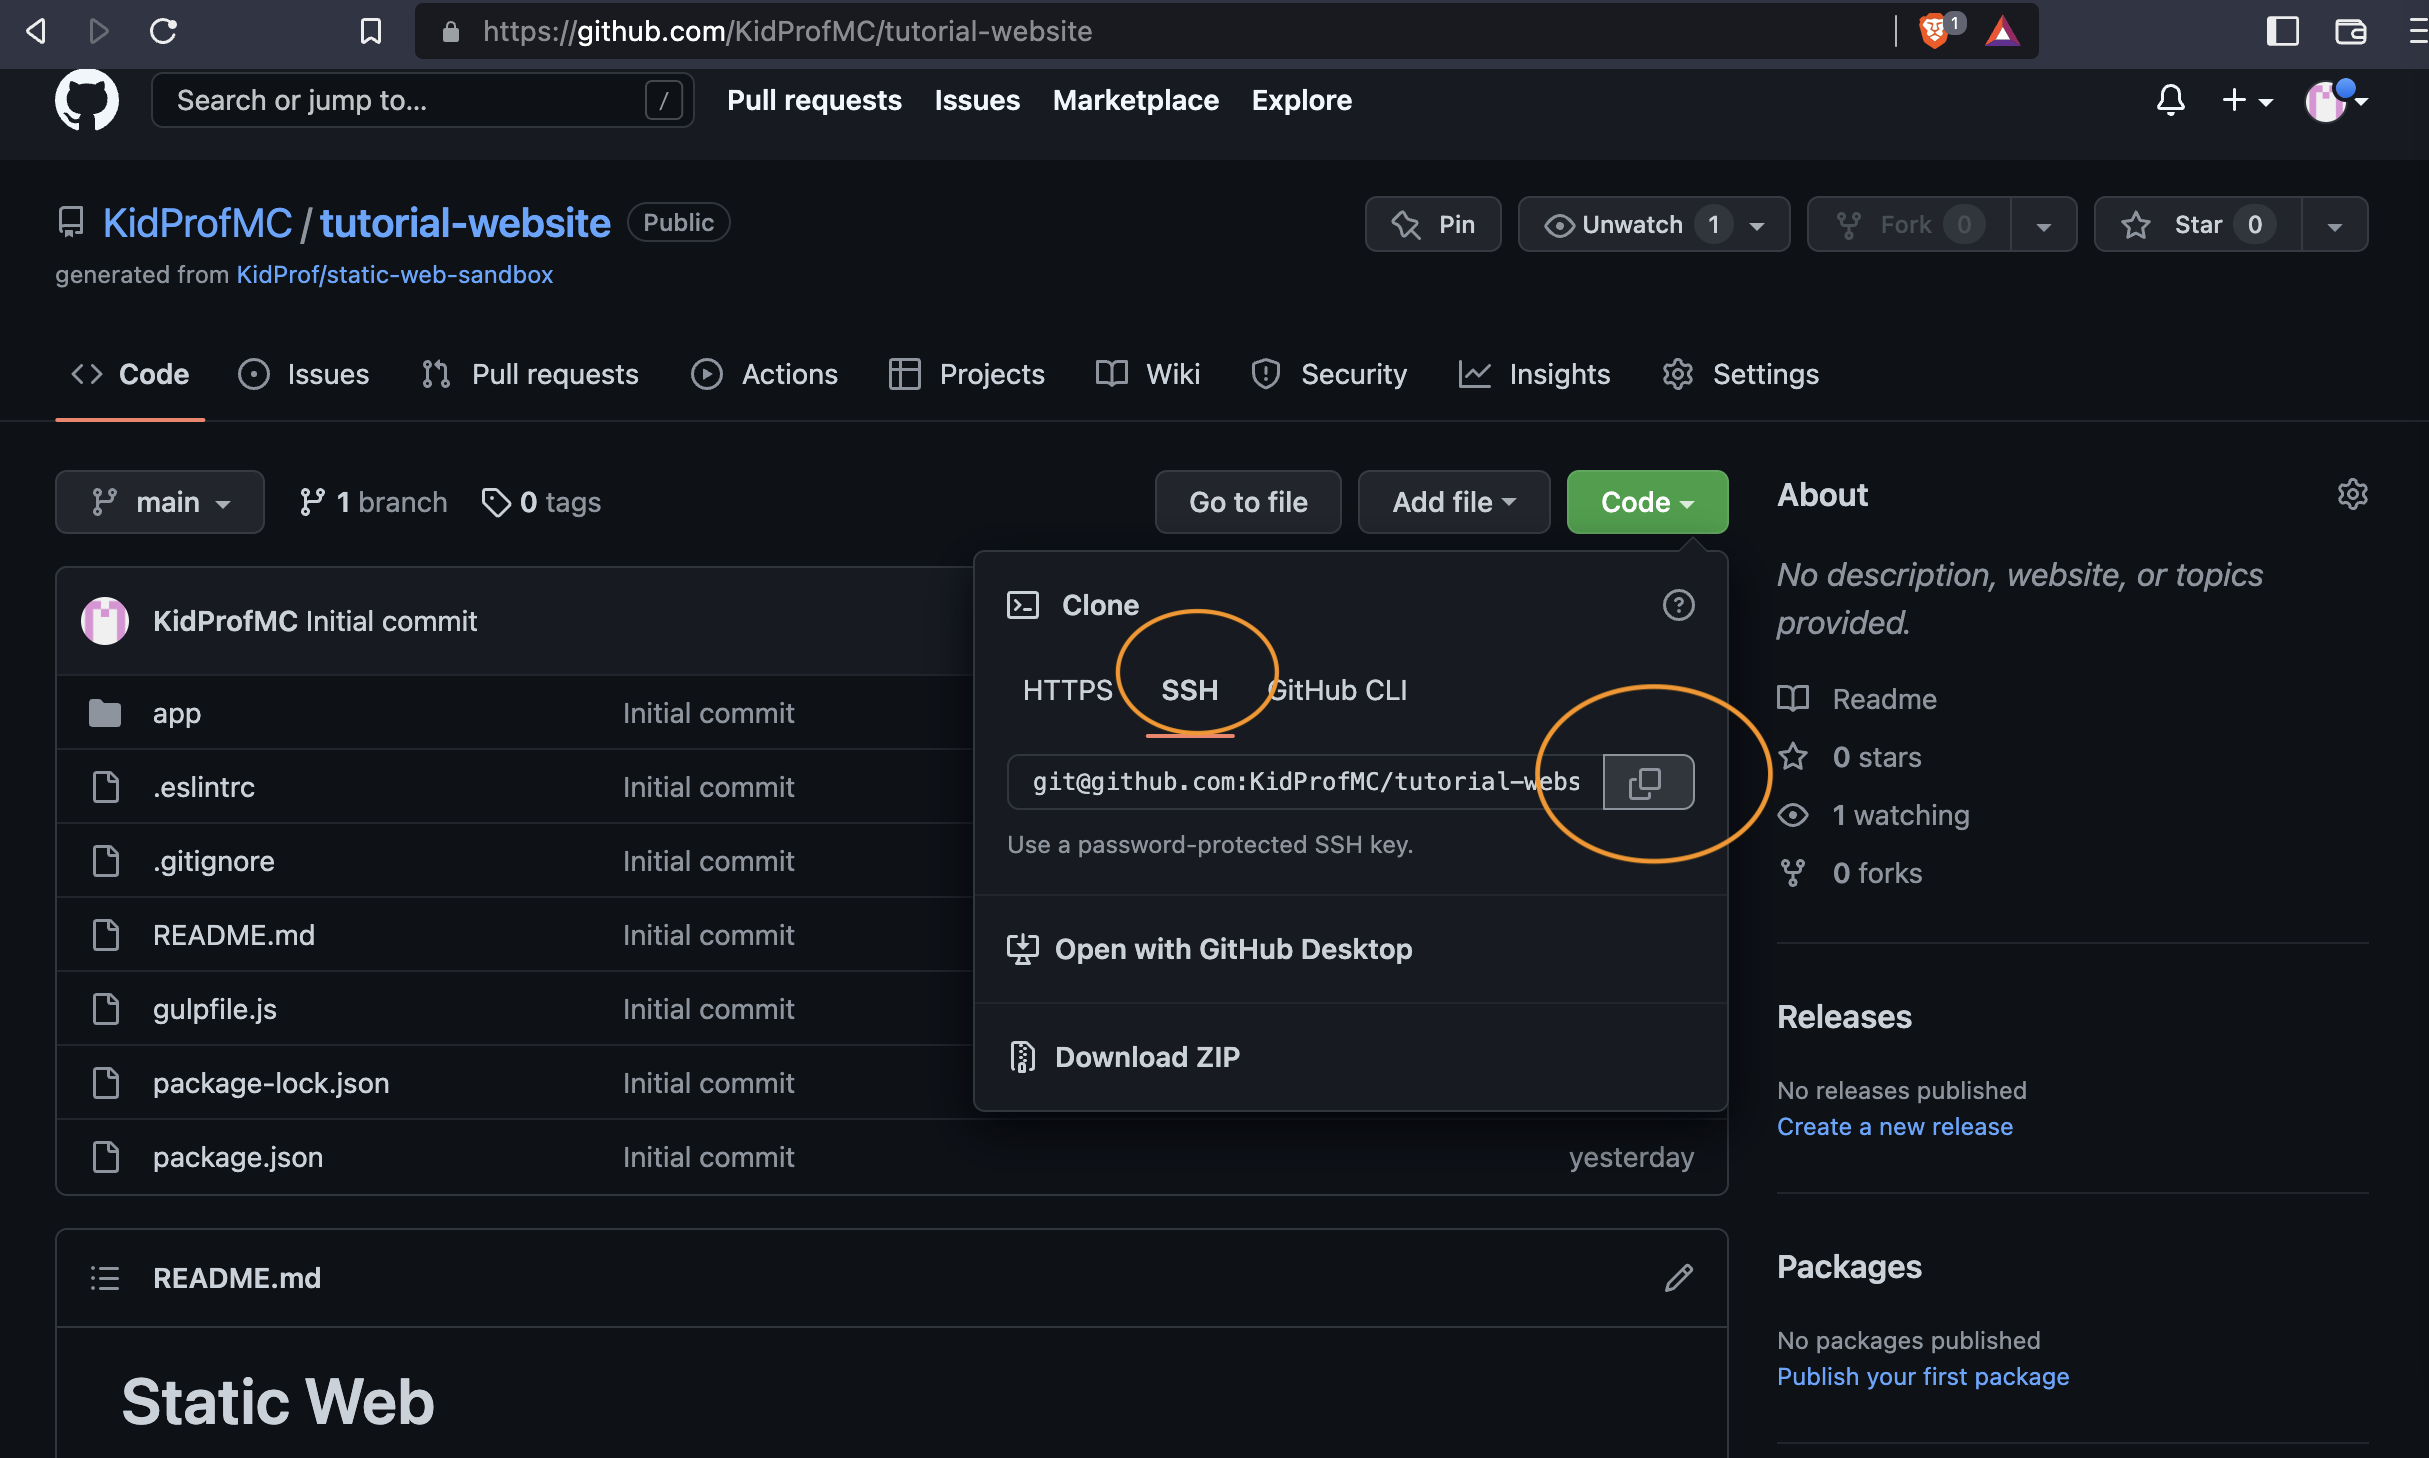
\includegraphics[width=15cm]{images/ch1-git-clone.png}
\caption{Getting the URL to download your project}
\label{fig:downloadbyssh}
\end{figure}

Use \texttt{git clone}, followed by pasting the URL obtained from GitHub. You should use your mouse to paste the URL in the classic way if you are on Windows or Linux, as \texttt{ctrl+V} would not work.\footnote{There is a shortcut, but specific to the machine. I will not bother to remember a new set of shortcuts.}

\section{Installing node.js}
\label{sec:install7}

Download node.js by following \href{https://nodejs.org/en/}{this link}.\footnote{Link: \url{https://nodejs.org/en/}} You should download the LTS\footnote{stands for long term support} version.

After installing, you can try running \texttt{node --version} in the command line.

\begin{lstlisting}[language=bash]
# If node is installed, it will show you the version number.
$ node --version
v16.14.0

# If node is not installed, it will show you an error message
$ node --version
zsh: command not found: node
\end{lstlisting}

\section{Installing dependencies for the project}

Open your command line, \texttt{cd} into the folder with the code in, run \texttt{npm install}. A new folder called \texttt{node\textunderscore modules} will be automatically created, with everything you need to use this project installed within that folder. (more in \cref{sec:quickstart})

\begin{lstlisting}[language=bash]
# KidProf in ~
$ cd code

# KidProf in ~/code
$ cd tutorial-website

# KidProf in ~/code/tutorial-website
$ npm install
\end{lstlisting}

\section{Opening the web page}

Run \texttt{npm run build} to build the web page. Again, more on this would be explained in \cref{sec:quickstart}.
\vspace{6mm}

\begin{lstlisting}[language=bash]
# KidProf in ~/code/tutorial-website on git:main 
$ npm run build

> static-web-sandbox@2.0.0 build
> gulp build

[09:56:22] Using gulpfile ~/code/tutorial-website/gulpfile.js
[09:56:22] Starting 'build'...
[09:56:22] Starting 'js'...
[09:56:22] Finished 'js' after 38 ms
[09:56:22] Starting 'pug'...
[09:56:22] Finished 'pug' after 83 ms
[09:56:22] Starting 'styling'...
[09:56:22] Finished 'styling' after 37 ms
[09:56:22] Starting 'imagecopy'...
[09:56:22] Finished 'imagecopy' after 2.67 ms
[09:56:22] Starting 'fontcopy'...
[09:56:22] Finished 'fontcopy' after 1.42 ms
[09:56:22] Finished 'build' after 164 ms
\end{lstlisting}
\vspace{6mm}

Then, open the folder containing the project in file explorer/ finder. Go to the \texttt{docs} folder, open \texttt{index.html} using a web browser of your choice. You should see something similar to \cref{fig:indexhtml}.

If you are unsure where your code is located, try running \texttt{pwd} in your command line, which should show you the full path that your code is in.
\vspace{6mm}

\begin{lstlisting}[language=bash]
# KidProf in ~/code/tutorial-website on git:main 
$ pwd
/Users/KidProf/code/tutorial-website
\end{lstlisting}

\begin{figure}[h]
\centering

\includegraphics[width=15cm]{images/ch1-indexhtml.png}
\caption{What index.html should look like}
\label{fig:indexhtml}
\end{figure}


\section{Installing VS Code}

Visual Studio Code (VS Code) is a text editor, with highlighted syntax and many more user-friendly features for you to code efficiently.

Download VS Code by following \href{https://code.visualstudio.com/}{this link}.\footnote{Link: \url{https://code.visualstudio.com/}}

\label{sec:pwdch1}
Then, open VS Code and open the folder containing the code. If you are unsure where your code is located, try running \texttt{pwd} in your command line, that should show you the full path that your code should be in.

\vspace{6mm}

This marks the end of the installation marathon. I hope you have learned some basic command line commands along the way, we will formally introduce them in \cref{sec:cmd}. The next two sections gives you a quick start guide to the project, so that you are well equipped for writing code in the second chapter.

\section{Quick start guide}
\label{sec:quickstart}

Long story short, there are two folders you need to concern about, the \texttt{app} folder and the \texttt{docs} folder. 

\begin{figure}[h]
\centering
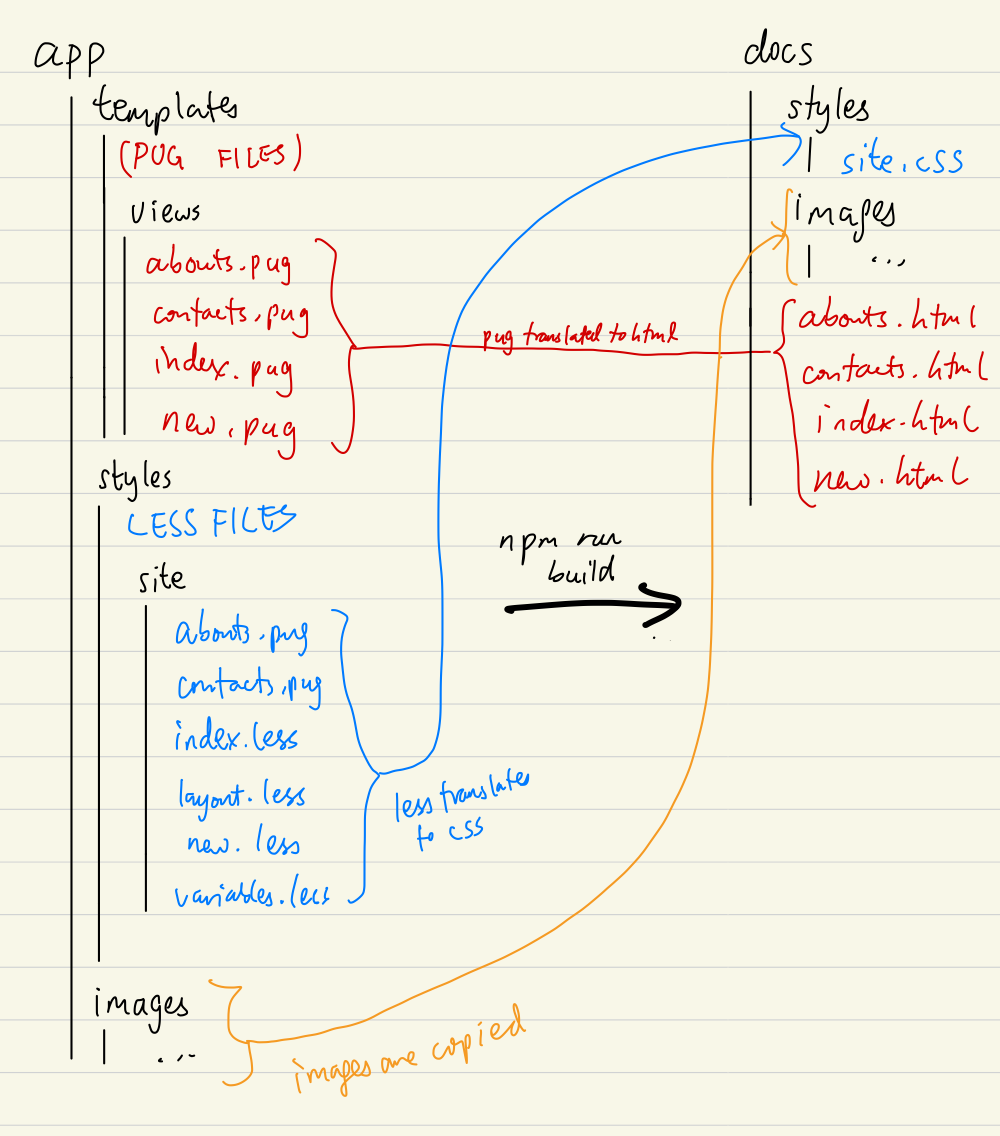
\includegraphics[width=13cm]{images/chn1-half-translation.png}
\caption{Overview of the translation process (quick start version)}
\end{figure}

The \texttt{app} folder is the one that we should work on, it includes the Pug files and much more. Pug files shapes the content of the web page. The Pug files that you should work up to chapter 5 are all under \texttt{app/templates/views}. Write your code inside the \texttt{.container} class, indented inwards. 
\vspace{6mm}

\begin{lstlisting}[language=pug]
extends ../layouts/default

block content
	.container
		//- Your code goes here...
\end{lstlisting}
\vspace{6mm}

You can open the HTML files in the \texttt{docs} folder using a browser of your choice. All files in the \texttt{docs} folder are generated based on our code in the \texttt{app} folder when we run \texttt{npm run build}. \textbf{IMPORTANT: Do NOT edit anything in the \texttt{docs} folder. Changes will be overwritten when you run \texttt{npm run build} again.}

The things you write in \texttt{app/templates/views} will be translated into an HTML file matching the name of the Pug file in the \texttt{docs} folder after you have run \texttt{npm run build}. For example, if you create a new file with the above template, called \texttt{new.pug} (You are advised to follow the above template when creating new Pug files under \texttt{app/templates/views}), then the content would appear when you open \texttt{docs/new.html} with your browser. 
\vspace{6mm}

At the same time, styling files are under \texttt{app/styles/site}, they are currently all empty and it is you job to fill them with amazing code in the later chapters :). They will be translated to \texttt{docs/site.css}.
\vspace{6mm}

Finally, when you run \texttt{npm run build}, the images under \texttt{app/images} folder would be copied to \texttt{docs/images}. That's why we can reference the images using \texttt{images/$<$filename$>$} in the Pug files, as we are referencing them in the perspective of the HTML files that are in the \texttt{docs} folder after the translation. 
\vspace{6mm}

There are a lot of things going on in this project, but this quick start guide should be enough for you to get started. More information about project structure would be in \cref{sec:projstructure}.

\section{VS Code tips}

You can run \texttt{code .} in your command line to open VS Code with the current directory in the command line opened, it is very convenient. If you can't get it to work, try setting up the environment variables as instructed \href{https://code.visualstudio.com/docs/setup/mac}{by this tutorial}\footnote{Link: \url{https://code.visualstudio.com/docs/setup/mac}}.
\vspace{6mm}

Another good tip is that you can highlight a few lines of text, and hit \texttt{tab}, and all those lines will be indented inwards; while hitting \texttt{shift+tab} will make them all indent outwards.
\vspace{6mm}

There are a number of extensions available in VS Code, but I think they are not necessary for beginners.

\section{Command line tips}

There are only two commands that you need to know in this stage - \texttt{ls} and \texttt{cd}. We have demonstrated \texttt{cd} earlier in \cref{sec:install5}.
\vspace{6mm}

\texttt{ls} stands for list. Lists out the files and folders you have in your current folder.
\vspace{6mm}

\begin{lstlisting}[language=bash]
$ ls
README.md   docs  node_modules  package.json    
app     gulpfile.js     package-lock.json
\end{lstlisting}